% TODO
\subsection{SOLID}
\subsubsection{Single Responsibility Principle}
Das Single Responsibility Principle (SRP) wird auch als Prinzip der einzigen Zuständigkeit bezeichnet. Dementsprechend soll eine Klasse nur einen Grund haben, um geändert werden zu müssen. Dadurch erhält jedes Objekt eine klar definierte Aufgabe. Durch das Anwenden dieses Prinzips, wird die Seperation of Concerns (SoC) umgesetzt. Sollte das Prinzip der Single Responsibility verletzt sein, so lässt sich dies relativ einfach mit der Antwort auf die Frage \glqq{}Was macht die Klasse?\grqq{} herausfinden. Sollte sich eine Konjunktion in der Antwort auf diese Frage befinden, kann man davon ausgehen, dass das SRP verletzt ist.

Als Beispiel für die Anwendung des SRP wird der ehemalige \texttt{MainController} betrachtet. Die Klasse als UML ist in Abbildung \ref{MainController} zu sehen. Auf die Frage \glqq{}Was macht die Klasse?\grqq{} lassen sich vier Antworten finden:
\begin{itemize}
\item Die generelle Logik, um den Hintergrund zu aktualisieren.
\item Das Halten und Verwalten des Timers für die zyklische Aktualisierung des Hintergrundbilds.
\item Die Logik, um das Hintergrundbild manuell in einem neuen Thread zu aktualisieren.
\item Das Weitergeben einer neuen Config zum Speichern bzw. das Abrufen der aktuellen Config (Adapter-Tätigkeit).
\end{itemize}

\begin{figure}[ht]
\centering
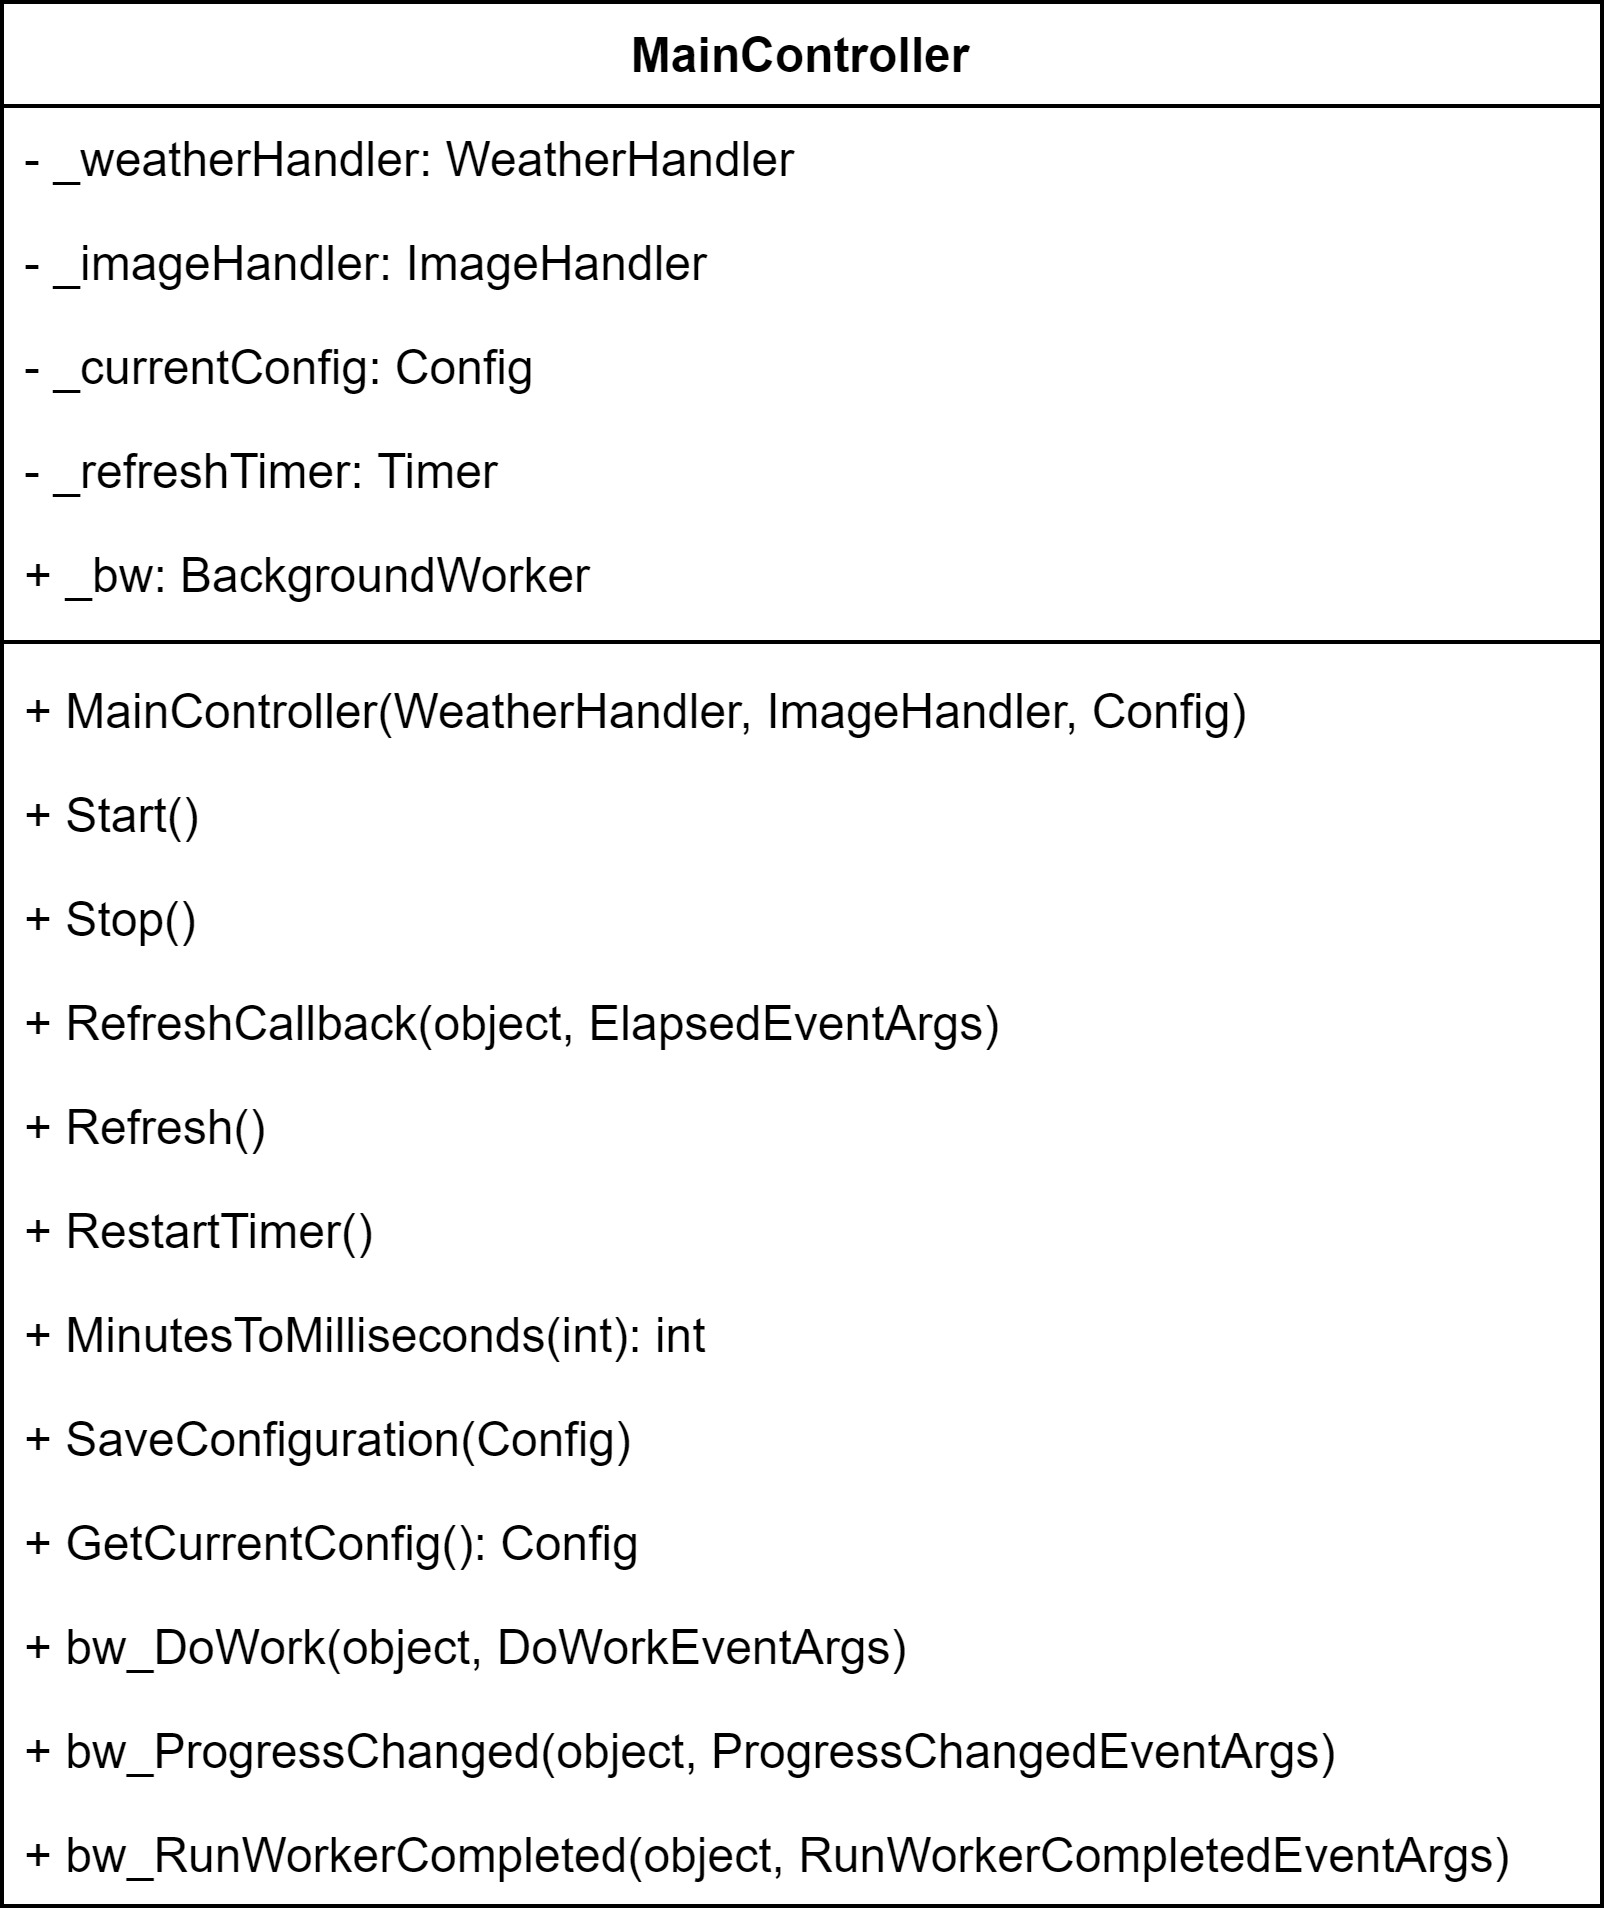
\includegraphics[width=0.5\textwidth]{Bilder/MainController}
\caption[Code Coverage Ergebnisse]{\label{MainController} MainController in UML-Form}
\end{figure}

Um diese verschiedenen Responsibilities in neue Klassen aufzuteilen wurden vier neue Klassen entwickelt. Diese werden im Folgenden kurz erläutert. Im \texttt{Refresher} ist die generelle Logik, um den Hintergrund zu aktualisieren ausgelagert. Der \texttt{UpdateTimer} übernimmt das zyklische Aktualisieren des Hintergunds und der \texttt{ScreenChangeWorker} das manuelle Aktualisieren im neuen Thread. In dem neuen \texttt{MainWindowController} wird das Weitergeben der GUI-Inputs an die inneren Schichten umgesetzt. Diese vier Klassen sind \href{https://github.com/Bronzila/WeatherWallpaper/blob/master/CleanArchitecturePics/Architektur_Vorher.jpg}{\color{blue}hier} auf dem UML-Diagramm der Anwendung zu erkennen. Hierbei ist erkennbar, dass der \texttt{MainWindowController}, durch seine Adaptertätigkeiten auch in die Adapter-Schicht bei der Clean Architecture übergegangen ist.

Dann noch ConfigHandler bzw Adapter und Zustand
\subsubsection{Open/Closed Principle}

\subsubsection{Liskov Substitution Principle}
Das Liskov Substitution Principle ist erfüllt, da abgesehen von den verwendeten Interfaces keine Vererbung verwendet wird.
\subsubsection{Interface Segregation Principle}

\subsubsection{Dependency Inversion Principle}

\subsection{GRASP}

\subsection{DRY}
